\documentclass[a4paper,oneside]{article}
\usepackage[french]{babel}
\usepackage[utf8]{inputenc}
\usepackage{hyperref} % références dans pdf
\usepackage[tt]{titlepic}
\usepackage{graphicx} % pour images
\usepackage{rotating} % pour
\usepackage{lmodern}
\usepackage{amsmath}
\usepackage{amssymb}
\usepackage{mathrsfs}
\usepackage{sistyle}
\usepackage{chngpage}
\usepackage{epstopdf}
\usepackage{gnuplottex}% pour faire du gnuplot directement dans le latex, finalement pas utilisé, résultats pas assez beaux
\usepackage[nottoc, notlof, notlot]{tocbibind} % pour que bibliographie soit comprise comme un chapitre ou section
\usepackage{appendix} % pour les annexes
\pagestyle{headings} % pour en têtes
\usepackage{mathenv}

\makeatletter % pour /bigcenter qui permet de s'affranchir des marges pour les images

\newskip\@bigflushglue \@bigflushglue = -100pt plus 1fil

\def\bigcenter{\trivlist \bigcentering\item\relax}
\def\bigcentering{\let\\\@centercr\rightskip\@bigflushglue%
\leftskip\@bigflushglue
\parindent\z@\parfillskip\z@skip}
\def\endbigcenter{\endtrivlist}

\makeatother

\begin{document}

%************************************************************************
%									TITRE
%************************************************************************


\begin{titlepage} % Suppresses headers and footers on the title page

	\centering % Centre everything on the title page

	\scshape % Use small caps for all text on the title page

	\vspace*{\baselineskip} % White space at the top of the page


	\rule{\textwidth}{1.6pt}\vspace*{-\baselineskip}\vspace*{2pt}
	 % Thick horizontal rule
	\rule{\textwidth}{0.4pt} % Thin horizontal rule

	\vspace{0.75\baselineskip} % Whitespace above the title

	{\LARGE RAPPORT DE VALIDATION :\\
	BUREAU D'\'ETUDES \\
	\vspace{0.75\baselineskip}
	Balistique \& Trajectoire} % Title

	\vspace{1\baselineskip} % Whitespace below the title
	\rule{\textwidth}{0.4pt}\vspace*{-\baselineskip}\vspace*{3.2pt}
	 % Thin horizontal rule
	\rule{\textwidth}{1.6pt} % Thick horizontal rule
	\vspace{2\baselineskip} % Whitespace after the title block

	%------------------------------------------------
	%	Subtitle
	%------------------------------------------------

	% Subtitle or further description
	Calculs Scientifiques \& Programmation

	\vspace*{3\baselineskip} % Whitespace under the subtitle

	%------------------------------------------------
	%	Editor(s)
	%------------------------------------------------


	\vspace{0.5\baselineskip} % Whitespace before the editors

	{\scshape\Large Quentin Bergé \\ Marc Ferrière} % Editor list

	\vspace{0.5\baselineskip} % Whitespace below the editor list

	\textit{ENSEEIHT} % Editor affiliation

	\vfill % Whitespace between editor names and publisher logo

	%------------------------------------------------
	%	Publisher
	%------------------------------------------------

	
\includegraphics[scale=0.3]{logoN7.png} % changer logo

	\vspace{0.3\baselineskip} % Whitespace under the publisher logo

Fevrier 2019 % Publication year



\end{titlepage}
\newpage

\tableofcontents
\newpage

%*******************************************************
% DEBUT RAPPORT
%********************************************************


\section{Introduction}
Il est question ici de créer un programme pour effectuer le calcul de trajectoire d'un objet en chute libre et propulsé selon l'enoncé proposé.
Dans ce rapport nous aborderons tout d'abord la modélisation du problème, puis nous nous focaliserons sur l'architecture du programme pour enfin aborder la validation.

\section{Modélisation}

\subsection{Chute Libre}

Si on effectue le bilan des forces sur un objet de masse $m$ possédant une vitesse initiale $v_0$ formant un angle $\alpha$ avec l'axe des abscisses à une altitude initiale $h$ :

\begin{equation*}
\Sigma \vec{F} = m \times \vec{a}
\end{equation*}

Ici $\vec{F}$ se limitera à $\vec{P} = m \vec{g}$ d'où $g=a$

\subsubsection{Solutions Analytiques}

On peut alors obtenir les équations analytiques avec $x(t)$ et $z(t)$ qui nous serviront de références :

\begin{align*}
x(t) &= v_0\cos(\alpha)t \\
z(t) &= v_0\sin(\alpha)t - \frac{gt^2}{2} + h\\
\end{align*}

On peut aussi obtenir les équations qui nous donneront la portée et le temps :

\begin{equation*}
portee = \frac{v_0}{g} \cos(\alpha) \sqrt{v_0 \sin(\alpha) +(v_0\sin(\alpha))^2 + 2gh}
\end{equation*}
\begin{equation*}
t_l = \frac{portee}{v_0\cos(\alpha)}	
\end{equation*}

\subsubsection{Modélisation Euler}
Le schéma d'Euler d'ordre 1 s'écrit : 

\begin{equation*}
y_{k+1} = y_{k}+ \Delta t \frac{df}{dt}(t_{k},y_{k})
\end{equation*}
On utilise un tableau de 4 colonnes noté $y$ :

\begin{equation*}
\begin{cases} 
y(1,i) = x(i)\\ 
y(2,i) = z(i)\\
y(3,i) = v_{x}(i)\\
y(4,i) = v_{z}(i)
\end{cases}
\end{equation*}

\[
\left\{
 \begin{array}{@{}r@{}}
  y(1,i) =  x(i)\\
  y(2,i) = z(i)\\
  y(3,i) = v_{x}(i)\\ 
  y(4,i) = v_{z}(i)\\
  \end{array}
\qquad
\Longleftrightarrow
\left\{
\begin{array}{@{}r@{}}
\frac{dx}{dt} = v_{x}\\
\frac{dz}{dt} = v_{z}\\
\frac{dv_{x}}{dt} = 0\\
\frac{dv_{z}}{dt} = -g\\  
\end{array}
\]

Ainsi on peut modéliser notre trajectoire de chute libre par un système du type : \label{1}

\begin{equation*}
\begin{cases} 
 y(3,i+1) = y(3,i)\\
 y(4,i+1) = y(4,i)  - dt\times g  \\
 y(1,i+1) = y(1,i)  + dt \times y(3,i)\\
 y(2,i+1) = y(2,i)  + dt \times y(4,i)\\
\end{cases}
\end{equation*}

A chaque pas de temps , on recalcule les vitesses et la position en $x$ et en $z$ à partir du système précédent.
  
\subsubsection{Modélisation Runge-Kutta d'ordre 4}
Le schéma de Runge-Kutta d'ordre 4 : \label{2}
\[
y_{k+1} = y_k + \frac{\Delta t}{6} ( k_1 + 2 k_2 + 2 k_3 + k4)
\]
Avec  : 
\begin{equation*}
\begin{cases} 
k_1 = \frac{dy_k}{dt}\\
k_2 = \frac{dy_k}{dt} + \frac{\Delta t }{2}\times k_1\\
k_3 = \frac{dy_k}{dt} + \frac{\Delta t }{2}\times k_2\\
k_4 = \frac{dy_k}{dt} + \Delta t \times k_3\\
\end{cases}
\end{equation*}

On utilise les dérivées de chute libre de la méthode Euler \ref{1} en appliquant la méthode Runge-Kutta à l'ordre 4 (\ref{2}). 


\subsection{Objet Portant Propulsé}

Maintenant notre masse est propulsé avec une force aérodynamique et on prend en compte la portance et la traînée dans nos calculs. 

\subsubsection{Méthode Euler}
On reprend le même schéma d'Euler à l'ordre 1 (\ref{1}) que pour la trajectoire en chute libre mais en intégrant les forces de portance $L$, de traînée $D$ et d'aérodynamique $F_0$
\label{3}
\[
\frac{dx}{dt} = v_{x}
\]
\[
\frac{dz}{dt} = v_{z}
\]
\[
\frac{dv_{x}}{dt} = \frac{  F_0 \cos(\theta) -L\sin(\theta) - D \cos(\theta) }{m}
\]
\[
\frac{dv_{z}}{dt} = \frac{ -g + F_0 \sin(\theta) +L\cos(\theta) - D \sin(\theta) }{m}
\]
 Avec $\theta $ l'angle entre entre les vecteurs vitesses  $v_x$ et $v_z$ : 
 \[
 \theta = \arctan(\frac{v_z}{v_x})
 \]
 \subsubsection{Méthode Runge-Kutta d'ordre 4}
 On reprend le schéma Runge-Kutta d'ordre 4 (\ref{2}) en modélisant les nouvelles dérivées vu en \ref{3}.
 
 
\section{Architecture}
Cette partie va détailler l'architecture du programme. 

\subsection{Contenu}

Le programme est placé dans le dossier \verb?Fortran? qui comprend :

\begin{itemize}
	\item un fichier \verb?mod_balistique.f90? % pour ne pas tenir compte de la mise en forme du texte très utile !!!
	\item un fichier de subroutines \verb?subroutines.f90?
	\item le programme \verb?main.f90?
	\item le fichier \verb?Makefile? permettant la compilation\\
	\end{itemize}

Le dossier \verb?RUN? comprend :
\begin{itemize}
	\item les fichier de sorties de forme \verb?BE_Methode_Modele_npt_XXXX_.out? et \verb? Paramétrisation_Alpha_Methode_Modele.out?
	\item le fichier d'entrée \verb?balistique.in?
	\item l'exécutable \verb?main.bin?\\
\end{itemize}

Dans le dossier \verb?Validation? sont compris :
\begin{itemize}
	\item les résultats du programme pour les différents modèles avec les deux modélisation
	\item les graphiques de résultats\\
\end{itemize}

Le dossier \verb?Rapport? comprend les ressources pour le rapport \LaTeX  ainsi que le rapport en lui-même.

\subsection{Algorithmie}
%algorithme du code à faire ou à mettre en annexe
Voici un algorigramme général présnetant le fonctionnement du programme :
\begin{figure}[h!]
\bigcenter

\centering
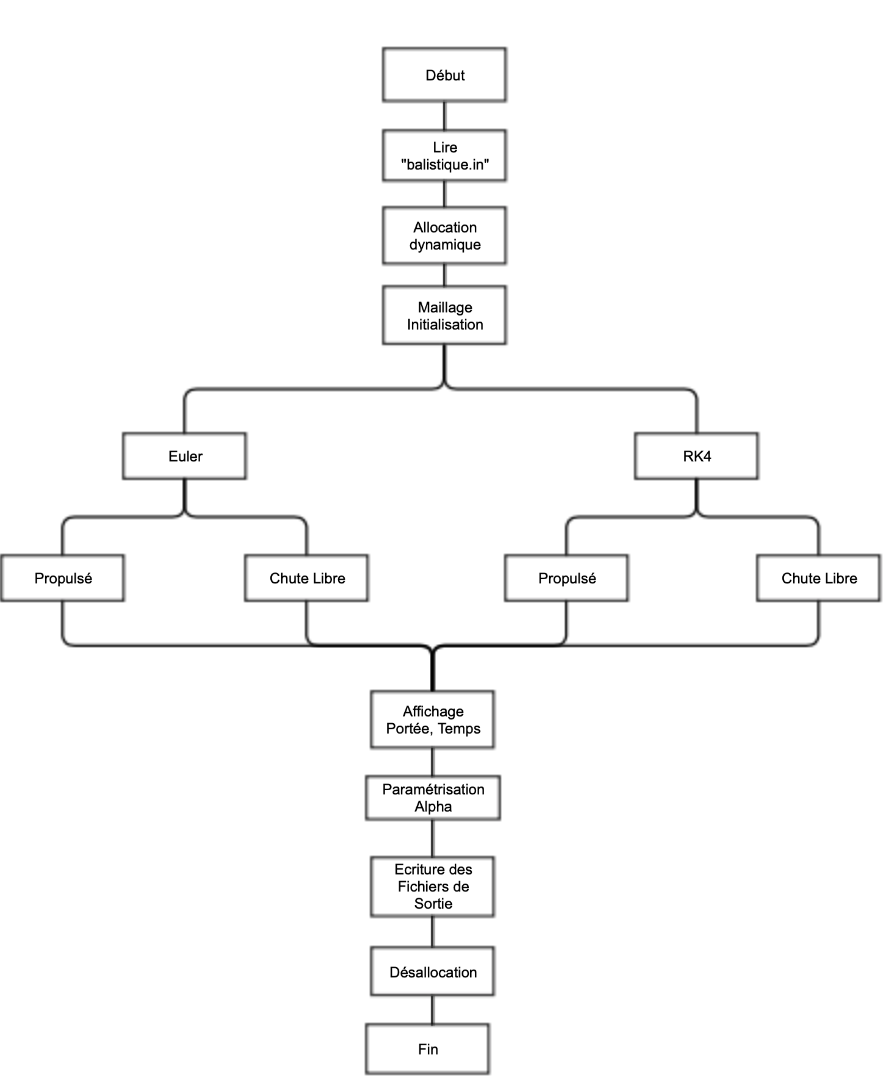
\includegraphics[scale=0.7] {algorigramme}
\caption{Algorigramme}	
\end{figure}

On détaille la procédure pour RK4 : 
\\

On a créer une subroutine nommée \verb?RK4? qui a pour paramètres d'entrées : 
\begin{itemize}
	\item dérivée de la fonction 
	\item n : numéro du vecteur qu'on veut calculer
\end{itemize}
Elle calcule la valeur du vecteur $y_{k+1}$ selon le schéma vu en \ref{2}. 
\\

Ensuite on appelle cette subroutine dans les 2 cas ( Chute libre ou Runge-Katta d'ordre 4 ) et selon les différentes forces qui s'appliquent, calcule les vecteurs positions et vitesses en x et en z. \\

Pour la variation de l'angle $\alpha$, la subroutine \verb?parametrisation_alpha? fait varier l'angle alpha de 25 $\degre$ jusqu'à 75 $\degre$ par pas de 5 $\degre$.\\
Ensuite cette subroutine reprend l'architecture du programme principal \verb?main.f90? pour calculer les trajectoires de chaque angle $alpha$.\\  
On affiche ensuite la portée et le temps de chute pour tous les angles. 




\section{Validation}

On effectue la validation selon la solution analytique pour le cas de la chute libre pour les deux méthodes.

Tout d'abord selon la méthode d'Euler.

\begin{figure}[h]
\centering
\begin{gnuplot}[terminal=latex]
set size 1,1; set title "Validation Chute Libre Euler";set xrange [0:180]; set yrange [0:140]; plot "BE_Euler_Chute_Libre_npt_10000.out" using 3:4 title "Méthode Euler" with lines, "BE_Euler_Chute_Libre_npt_10000.out" using 5:6 title "Méthode Analytique" with lines
\end{gnuplot}
\caption{Validation de la Chute Libre selon la méthode d'Euler avec la méthode Analytique}
\end{figure}

On observe la parfaite superposition entre les deux courbes, ainsi on peut valider nos résultats avec la résolution de la méthode d'Euler.

\begin{figure}[h!]
\centering
\begin{gnuplot}[terminal=latex]
set size 1,1; set title "Validation Chute Libre RK4";set xrange [0:180]; set yrange [0:140]; plot "BE_RK4_Chute_Libre_npt_10000.out" using 3:4 title "Méthode RK4" with lines, "BE_RK4_Chute_Libre_npt_10000.out" using 5:6 title "Méthode Analytique" with lines
\end{gnuplot}
\caption{Validation de la Chute Libre selon la méthode RK4 avec la méthode Analytique}
\end{figure}

\begin{figure}[h!]
\centering
\begin{gnuplot}[terminal=latex]
set size 1,1; set title "Validation Propulsé RK4 Euler";set xrange [0:370]; set yrange [0:140]; plot "BE_RK4_Propulsé_npt_10000.out" using 3:4 title "Méthode RK4" with lines, "BE_Euler_Propulsé_npt_10000.out" using 3:4 title "Méthode Euler" with lines
\end{gnuplot}
\caption{Validation du modèle Propulsé selon la méthode RK4 et la méthode Euler}
\end{figure}

\newpage

\section{Conclusion}


\end{document}
